\documentclass{article}
\usepackage[T1]{fontenc}
\usepackage[latin9]{inputenc}
\usepackage{amstext}
\usepackage{graphicx}
\usepackage{esint}

\title{How an IQ mixer Works}
\date{22 February 2010}
\author{Daniel Sank}

\begin{document}

\maketitle

\begin{abstract}
We use IQ mixers in the lab to generate arbitrary waveforms to control
the qubits. In this note I show how the mixer works, and in particular
that it can be used to generate arbitrary waveforms with bandwidth
centered around the input RF carrier frequency, and with total bandwidth
of twice that of the DACs driving the I and Q channels. 
\end{abstract}

\section{Why an IQ mixer?}

An IQ mixer is essentially a device that can do phase sensitive sideband
mixing. To understand what that means let's look at what happens when
we try to change the frequency of a carrier signal by using a single
mixer. We have an RF source $\cos(\Omega t)$, and a modulating signal
$m(t)=\cos(\omega t+\phi)$ where $\omega<\Omega$. For example the
carrier frequency $\Omega$ could be something like 1GHz, and the
modulating frequency $\omega$ might be 10 MHz. If we pass these signals
through a mixer we get\begin{eqnarray*}
\textrm{signal} & = & \cos(\Omega t)\cos(\omega t+\phi)\\
\textrm{signal} & = & \frac{1}{2}\left(\cos\left[\left(\Omega-\omega\right)t-\phi\right]+\cos\left[\left(\Omega+\omega\right)t+\phi\right]\right)\end{eqnarray*}
 We get two output signals, one with frequency above the carrier and
one below. By controlling the modulation frequency $\omega$ and phase
$\phi$ we can control the output frequency and phase. However, just
using those two controls we can't get rid of the fact that we always
get two sinusoids at the output. Even if we were to additionally control
the amplitude of the modulating signal we would always get two outputs
centered at $\Omega-\omega$ and $\Omega+\omega$ in frequency, which
are called the two $\emph{sidebands}$.

To find out how much control we really have let's see what happens
if we consider a modulating signal that is an arbitrary, but bandlimited,
function of time,\[
m(t)=\int_{0}^{BW}m(\omega)\cos\left[\omega t+\phi(\omega)\right]\]
 This is the Fourier representation of a real signal. Note that $m(\omega)$
is real. Then the output of the mixer, $s(t)$, will be (ignoring
prefactors)\begin{eqnarray*}
s(t) & = & \int_{0}^{BW}m(\omega)\cos\left[\Omega t\right]\cos\left[\omega t+\phi(\omega)\right]\\
s(t) & = & \int_{0}^{BW}m(\omega)\cos\left[\left(\Omega+\omega\right)t+\phi(\omega)\right]+\cdots\\
 &  & \cdots+m(\omega)\cos\left[\left(\Omega-\omega\right)t-\phi(\omega)\right]\end{eqnarray*}
 For each frequency $\omega$ you can choose $m$ and $\phi$ so that
the up or down converted term has the amplitude and phase that you
want. However, you can't simultaneously control both. This means that
you could generate an arbitrary waveform with frequency components
in the range $\left[\Omega,\Omega+BW\right]$ as long as you filter
away the stuff in the range $\left[\Omega-BW,\Omega\right]$. This
is where the IQ mixer comes in.


\section{How it works}

The basic layout of the mixer is shown in Figure 1. The RF input is
supplied by a microwave source, in our case the Anritsu, and the modulating
signals $I(t)$ and $Q(t)$ come from the GHz DACs. %
\begin{figure}
\includegraphics[scale=0.5]{diagram}
\caption{The block diagram on an IQ mixer}
\end{figure}

Consider as a first case, what happens if we take $I(t)=\cos(\omega t+\phi)$
and $Q(t)=-\sin(\omega t+\phi)$. Then the output signal is (again,
leaving out all prefactors),\begin{eqnarray*}
s(t) & = & \cos(\Omega t)\cos(\omega t+\phi)-\sin(\Omega t)\sin(\omega t+\phi)\\
s(t) & = & \cos\left[\left(\Omega+\omega\right)t+\phi\right]+\cos\left[\left(\Omega-\omega\right)t-\phi\right]+\cdots\\
 &  & \cdots+\cos\left[\left(\Omega+\omega\right)t+\phi\right]-\cos\left[\left(\Omega-\omega\right)t-\phi\right]\\
s(t) & = & \cos\left[\left(\Omega+\omega\right)t+\phi\right]\end{eqnarray*}
 You can see that we've arrived with an output signal that has controllable
phase and frequency, with no other sideband present. This is the point
of an IQ mixer. The existence of the phase shifted quadrature from
the RF carrier allows us to cancel out the unwanted sideband.

Now let's see what we can do if $I(t)$ and $Q(t)$ are arbitrary
band limited signals,\begin{eqnarray*}
I(t) & = & \int_{0}^{BW}I(\omega)\cos\left(\omega t+\phi_{I}(\omega)\right)\\
Q(t) & = & \int_{0}^{BW}Q(\omega)\sin\left(\omega t+\phi_{Q}(\omega)\right)\end{eqnarray*}
 The signal output in this case is\begin{eqnarray*}
s(t) & = & \int_{0}^{BW}\\
 & I(\omega) & \left\{ \cos\left[\left(\Omega+\omega\right)t+\phi_{I}(\omega)\right]+\right.\\
 &  & \left.\cos\left[\left(\Omega-\omega\right)t-\phi_{I}(\omega)\right]\right\} +\cdots\\
 & Q(\omega) & \left\{ -\cos\left[\left(\Omega+\omega\right)t+\phi_{Q}(\omega)\right]+\right.\\
 &  & \left.\cos\left[\left(\Omega-\omega\right)t-\phi_{Q}(\omega)\right]\right\} \end{eqnarray*}
 In order to generate an arbitrary signal we need to be able to control
the amplitude and phase of each frequency component. Notice that for
fixed $\omega$ the integrand involves terms with frequencies $\Omega+\omega$
and $\Omega-\omega$. That means that for each $\omega$ we have to
pick our control parameters such that we get the amplitude and phase
at both of these sidebands correct simultaneously. You can see that
this is possible through the following argument. At each frequency
we have to get both sidebands right, and each one has amplitude and
phase. That means there are four paramters per frequency. Since for
each frequency we can control $I$, $Q$, $\phi_{I}$ and $\phi_{Q}$,
we have as many controls as there are parameters. Therefore, we can
control everything we need to generate an arbitrary waveform with
frequency components in the range $\left[\Omega-\omega,\Omega+\omega\right]$.


\section{Complex form}

The mathematics is much simpler if we use complex numbers. An arbitrary
bandlimited waveform can be written\[
f(t)=\int_{-BW}^{BW}f(\omega)e^{i\omega t}d\omega\]
 with the constraint that $f(-\omega)=f^{*}(\omega)$. Using this
form we rewrite our control signals as\begin{eqnarray*}
I(t) & = & \int_{-BW}^{BW}I(\omega)e^{i\omega t}d\omega\\
Q(t) & = & \int_{-BW}^{BW}Q(\omega)e^{i\omega t}d\omega\end{eqnarray*}
 where now $I$, and $Q$ are complex. Channel $I$ gets multiplied
by the cosine term of the carrier, and channel $Q$ gets multiplied
by the sine term, so the outputs of the mixers are\begin{eqnarray*}
I(t)\cos(\Omega t) & = & \int I(\omega)\left[e^{i\left(\omega+\Omega\right)t}+e^{i\left(\omega-\Omega\right)t}\right]d\omega\\
\textrm{and}\; Q(t)\sin(\Omega t) & = & \int Q(\omega)\left[-ie^{i\left(\omega+\Omega\right)t}+ie^{i\left(\omega-\Omega\right)t}\right]d\omega\end{eqnarray*}
 Summing the first term in each integral gives\begin{eqnarray*}
s_{1}(t) & = & \int_{-BW}^{BW}\left[I\left(\omega\right)-iQ(\omega)\right]e^{i(\omega+\Omega)t}d\omega\\
s_{1}(t) & = & \int_{\Omega-BW}^{\Omega+BW}\left[I\left(\omega-\Omega\right)-iQ\left(\omega-\Omega\right)\right]e^{i\omega t}d\omega\end{eqnarray*}
 Similarly, summing the second terms gives\begin{eqnarray*}
s_{2}(t) & = & \int_{-\Omega-BW}^{-\Omega+BW}\left[I\left(\omega+\Omega\right)+iQ\left(\omega+\Omega\right)\right]e^{i\omega t}d\omega\end{eqnarray*}
 Change variables $\omega\rightarrow-\omega$,\begin{eqnarray*}
s_{2}(t) & = & \int_{\Omega-BW}^{\Omega+BW}\left[I\left(-\omega+\Omega\right)+iQ\left(-\omega+\Omega\right)\right]e^{-i\omega t}d\omega\end{eqnarray*}
 and then use the fact that $I(\omega)=I(-\omega)^{*}$ and $Q(\omega)=Q(-\omega)^{*}$,
\[
s_{2}(t)=\int_{\Omega-BW}^{\Omega+BW}\left[I^{*}\left(\omega-\Omega\right)+iQ^{*}\left(\omega-\Omega\right)\right]e^{-i\omega t}d\omega\]
 Now add the two parts of the signal together,\begin{eqnarray*}
s(t) & = & \int_{\Omega-BW}^{\Omega+BW}d\omega\\
 &  & \left[I\left(\omega-\Omega\right)-iQ\left(\omega-\Omega\right)\right]e^{i\omega t}+\\
 &  & \left[I^{*}\left(\omega-\Omega\right)+iQ^{*}\left(\omega-\Omega\right)\right]e^{-i\omega t}\\
s(t) & = & \int_{\Omega-BW}^{\Omega+BW}d\omega s(\omega)e^{i\omega t}+s^{*}(\omega)e^{-i\omega t}\end{eqnarray*}
 where $s(\omega)=I(\omega-\Omega)-iQ(\omega-\Omega)$. This is exactly
the equation for the Fourier transform of an arbitrary real signal
$s(t)$ with frequency components in $\left[\Omega-BW,\Omega+BW\right]$.
In the lab we usually know what signal $s(t)$ we want to send to
the qubit. The question then is, how do we pick $I(t)$ and \textbf{$Q(t)$
}to generate a chosen $s(t)$? To answer this we can work through
how choose $I$ and $Q$ to acheive specific values of $s$ at frequencies
$\Omega+\omega$ and $\Omega-\omega$.\begin{eqnarray*}
s^{+}\equiv s(\Omega+\omega) & = & I(\omega)-iQ(\omega)\\
\textrm{and}\quad s(\Omega-\omega) & = & I(-\omega)-iQ(-\omega)\\
s^{-}\equiv s(\Omega-\omega) & = & I^{*}(\omega)-iQ^{*}(\omega)\end{eqnarray*}
 since $I(t)$ and $Q(t)$ are real. Breaking things up into real
and imaginary parts we get\begin{eqnarray*}
\Re s^{+} & = & \Re I+\Im Q\\
\Im s^{+} & = & \Im I-\Re Q\\
\Re s^{-} & = & \Re I-\Im Q\\
\Im s^{-} & = & -\Im I-\Re Q\end{eqnarray*}
 Inverting these equations gives equations for the real and imaginary
parts of $A$ and $B$\begin{eqnarray*}
\Re I & = & \Re s^{+}+\Re s^{-}\\
\Im I & = & \Im s^{+}-\Im s^{-}\\
\Re Q & = & -\Im s^{+}-\Im s^{-}\\
\Im Q & = & \Re s^{+}-\Re s^{-}\end{eqnarray*}
 These equations tell you how to choose $I$ and $Q$ to acheive the
upconverted signal $s(t)$ that you want. These are the equations
you would use if you wanted a program to compute $A$ and $B$ for
a desired $s(t)$. You Fourier transform $s(t)$, split it into real
and imaginary parts, construct $I$ and $Q$, and then inverse Fourier
transform to get $I(t)$ and $Q(t)$.

We check this result with an example signal,\begin{eqnarray*}
s(t) & = & \cos\left[\left(\Omega+\omega\right)t+\phi\right]+\cos\left[\left(\Omega-\omega\right)t+\theta\right]\\
s(t) & = & e^{i\phi}e^{i(\Omega+\omega)t}+e^{-i\phi}e^{-i(\Omega+\omega)t}+\cdots\\
 &  & \cdots+e^{i\theta}e^{i(\Omega-\omega)t}+e^{-i\theta}e^{-i(\Omega-\omega)t}\\
s(t) & = & e^{i\phi}e^{i(\Omega+\omega)t}+e^{i\theta}e^{i(\Omega-\omega)t}+\textrm{complex conjugate}\end{eqnarray*}
 According to our formulae then we have\begin{eqnarray*}
\Re I & = & \cos(\phi)+\cos(\theta)\\
\Im I & = & \sin(\phi)-\sin(\theta)\\
\Re Q & = & -\sin(\phi)-\sin(\theta)\\
\Im Q & = & \cos(\phi)-\cos(\theta)\end{eqnarray*}
 Now we convert $A$ and $B$ to the time domain.\begin{eqnarray*}
I(t) & = & \left\{ \left[\cos(\phi)+\cos(\theta)\right]+i\left[\sin(\phi)-\sin(\theta)\right]\right\} e^{i\omega t}\\
 &  & +c.c.\\
I(t) & = & \left[\cos(\phi)+\cos(\theta)\right]\cos\left(\omega t\right)\cdots\\
 &  & \cdots-\left[\sin(\phi)-\sin(\theta)\right]\sin\left(\omega t\right)\end{eqnarray*}
 and similarly\begin{eqnarray*}
Q(t) & = & \left\{ -\left[\sin(\phi)+\sin(\theta)\right]+i\left[\cos(\phi)-\cos(\theta)\right]\right\} e^{i\omega t}\\
 &  & +c.c.\\
Q(t) & = & -\left[\sin(\phi)+\sin(\theta)\right]\cos\left(\omega t\right)\cdots\\
 &  & \cdots-\left[\cos(\phi)-\cos(\theta)\right]\sin\left(\omega t\right)\end{eqnarray*}
 Finally we compute $s(t)$. To simplify notation we use $\cos(+)\equiv\cos\left(\left(\Omega+\omega\right)t\right)$
and $\cos(-)\equiv\cos\left(\left(\Omega-\omega\right)t\right)$ etc.
First the $I$ part, \begin{eqnarray*}
I(t)\cos\left(\Omega t\right) & = & \left[\cos(\phi)+\cos(\theta)\right]\cos\left(\omega t\right)\cos\left(\Omega t\right)\cdots\\
 &  & -\left[\sin(\phi)-\sin(\theta)\right]\sin\left(\omega t\right)\cos\left(\Omega t\right)\\
I(t)\cos\left(\Omega t\right) & = & \left[\cos(\phi)+\cos(\theta)\right]\left[\cos(-)+\cos(+)\right]\cdots\\
 &  & -\left[\sin(\phi)-\sin(\theta)\right]\left[\sin(+)-\sin(-)\right]\end{eqnarray*}
 and now the $B$ part\begin{eqnarray*}
Q(t)\sin\left(\Omega t\right) & = & -\left[\sin(\phi)+\sin(\theta)\right]\cos\left(\omega t\right)\sin\left(\Omega t\right)\cdots\\
 &  & -\left[\cos(\phi)-\cos(\theta)\right]\sin\left(\omega t\right)\sin\left(\Omega t\right)\\
Q(t)\sin\left(\Omega t\right) & = & -\left[\sin(\phi)+\sin(\theta)\right]\left[\sin(+)+\sin(-)\right]\cdots\\
 &  & -\left[\cos(\phi)-\cos(\theta)\right]\left[\cos(-)-\cos(+)\right]\end{eqnarray*}
 Adding together the $\Omega+\omega$ terms gives \begin{eqnarray*}
\cos(+)\cos(\phi)-\sin(+)\sin(\phi) & = & \cos\left(\left(\Omega+\omega\right)t+\phi\right)\end{eqnarray*}
 and adding the $\Omega-\omega$ terms gives\[
\cos(-)\cos(\theta)-\sin(-)\sin(\theta)=\cos\left(\left(\Omega-\omega\right)t+\theta\right)\]
 yielding\[
s(t)=\cos\left(\left(\Omega+\omega\right)t+\phi\right)+\cos\left(\left(\Omega-\omega\right)t+\theta\right)\]
 which is what we wanted. This shows that the equations we gave for
$I$ and $Q$ are correct (although we didn't check amplitudes here...
exercise for the reader). 
\end{document}
